%% ------------------------------------------------------------------------- %%
\chapter{Resultados}
\label{cap:resultados}
    
    Para tratamento dos dados, foram avaliadas as diferentes perguntas relacionadas a um mesmo contexto. Este contexto variava desde grupos de funcionalidades até a informações pessoais do usuário. 
    
    As perguntas da maior parte dos grupos de funcionalidades abordavam alguns parâmetros e, a fim de priorizar as funcionalidades de cada grupo, fez-se necessária a criação de um índice estatístico, que será descrito no decorrer desta seção.  Analisando o resultado das perguntas referentes ao perfil dos membros da rede, algumas observações interessantes puderam ser feitas, como realatado a seguir.

\section{Alguns fatos observados}
\label{sec:observacoes}

    A partir dos dados recolhidos, foi possível identificar diversas características sobre o perfil dos usuários que utilizam a rede. Uma delas é que aproximadamente metade dos participantes são da área de humanas, enquanto os estudantes da área de biológicas e de exatas representaram, cada grupo, cerca de um quarto das respostas, como mostra a Figura~\ref{fig:chart-area}.
    
\begin{figure}[!h]
  \centering
  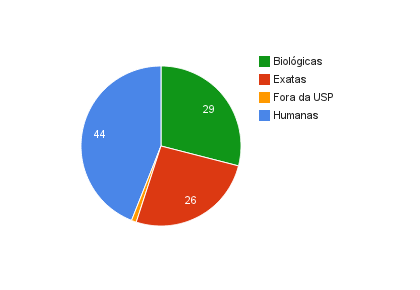
\includegraphics[width=.60\textwidth]{chart-area.png} 
  \caption{Área de estudo dos participantes}
  \label{fig:chart-area} 
\end{figure}
Outra observação é que, considerando o primeiro acesso do usuário na rede, a proporção de usuários interessados no formulário foi a mesma para os seguintes grupos: primeiro acesso há um mês; há um ano; há mais de um ano, como indica a Figura~\ref{fig:chart-firstcontact}.
    
\begin{figure}[!h]
  \centering
  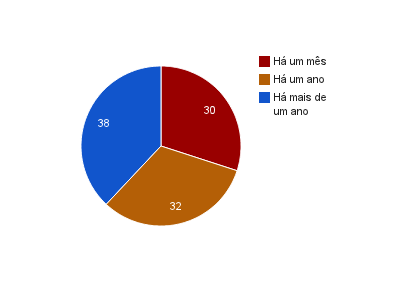
\includegraphics[width=.60\textwidth]{chart-firstcontact.png} 
  \caption{Momento do primeiro contato com a rede}
  \label{fig:chart-firstcontact} 
\end{figure}
Uma informação muito relevante sobre o uso do Stoa é o fato de mais de três quartos dos participantes registrarem-se na rede devido à solicitação de um professor, e, por isso, aproximadamente metade dos usuários utilizam a rede principalmente para atividades relacionadas a uma disciplina acadêmica.

%área; tempo desde primeiro acesso

\section{Índice estatístico}
\label{sec:indice}

    Foram feitas parametrizações com as marcações "melhor", "pior" e "maior uso" em determinados grupos de funcionalidades e, para esses recursos serem priorizados dentro do respectivo grupo, um índice apropriado foi estabelecido. Para a classificação, os requisitos para este índice exigiam que as funcionalidades com os parâmetros "pior" e "melhor" recebessem valores bem distintos e que fossem diferenciadas das demais. Além disso, a funcionalidade com o parâmetro "maior uso" deveria receber uma importância positiva, pois era utilizada mais que as demais funcionalidades de seu grupo.
    
    Com as considerações acima apontadas, foi elaborado o seguinte índice:
    \begin{itemize}
    \item 
    Em um determinado grupo de funcionalidades, para o conjunto de respostas de cada usuário, foi feita a seguinte lógica:
    
        \begin{itemize}
        \item  
        Atribuir 3 à funcionalidade escolhida para "a melhor"
        \item
        Atribuir 0 à funcionalidade escolhida para "a pior"
        \item
        Atribuir 1 às demais funcionalidades
        \item
        Atribuir um peso de 1.2 à funcionalidade escolhida para "maior uso"
        \end{itemize}
    \item 
    Em seguida, para cada funcionalidade, foi calculada a média de todos os valores associados às respostas dos usuários.
    \item 
    Com esta média, tornou-se possível ordenar as funcionalidades de acordo com a opinião dos usuários.
    \end{itemize}
    
    
\section{Priorização das questões}
\label{sec:priorizacao}

    O índice descrito na seção anterior,~\ref{sec:indice} não pôde, no entanto, ser empregado a todos os grupos de funcionalidades, pois algumas funcionalidades não podiam ser comparadas com outras, como no caso da ferramenta \emph{Google Analytics}. Os grupos de funcionalidades submetidos ao índice foram: i, v, vi; e, para cada grupo, a média de cada funcionalidade, assim como a ordenação, podem ser vistas nas tabelas a seguir:

\begin{figure}[!h]
  \centering
  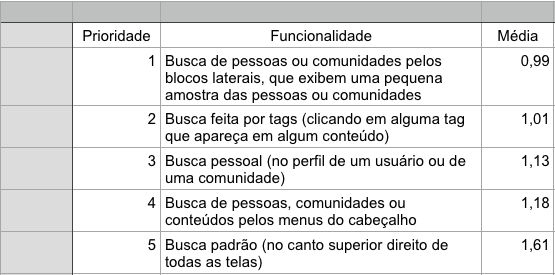
\includegraphics[width=.40\textwidth]{grupo-i.png} 
  \caption{Funcionalidades do grupo i}
  \label{fig:grupo-i} 
\end{figure}

    
\begin{figure}[!h]
  \centering
  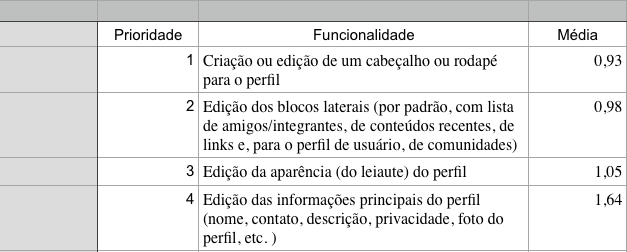
\includegraphics[width=.40\textwidth]{grupo-v.png} 
  \caption{Funcionalidades do grupo v}
  \label{fig:grupo-v} 
\end{figure}

    
\begin{figure}[!h]
  \centering
  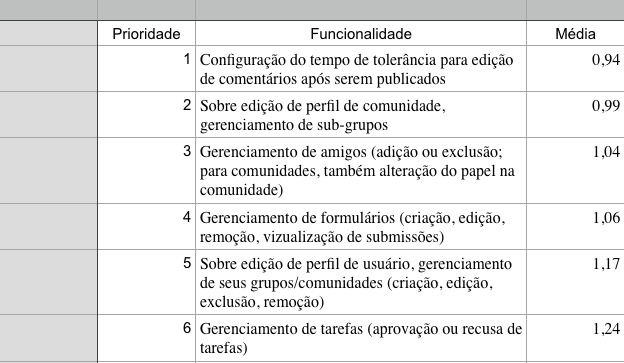
\includegraphics[width=.40\textwidth]{grupo-vi.png} 
  \caption{Funcionalidades do grupo vi}
  \label{fig:grupo-vi} 
\end{figure}


    Para a classificação geral, não foi possível comparar funcionalidades de grupos diferentes, pois o usuário não respondeu às perguntas dentro deste contexto. Por isso, foi selecionado o recurso considerado o pior pela ordenação de cada um dos grupos acima citados: 
    \begin{itemize}
    \item Busca de pessoas ou comunidades pelos blocos laterais, que exibem uma pequena amostra das pessoas ou comunidades - Grupo i
    \item Criação ou edição de um cabeçalho ou rodapé para o perfil - Grupo v
    \item Configuração do tempo de tolerância para edição de comentários após serem publicados - Grupo vi
    \end{itemize}
    Para os demais grupos, quando adequado, foi analisada separadamente a pergunta feita a ele. Em seguida, as funcionalidades foram ordenadas de acordo com as respostas e a primeira de cada ordenação foi selecionada. Do grupo xii, porém, foram selecionadas as duas primeiras da lista, pois a pergunta referente ao grupo fornecia um retorno mais preciso sobre a usabilidade da funcionalidade. Essa análise levou à inclusão dos seguintes recursos à lista:
    \begin{itemize}
    \item Quem somos (link rodapé) - Grupo ii
    \item Acesso ao Painel de Controle pelo link abaixo da foto do usuário logado em alguma página de seu perfil - Grupo iv
    \item Botões para ações em conteúdos - Grupo xii
    \end{itemize}
    Os grupos vii e ix continham apenas uma funcionalidade, no entanto, elas se mostraram muito interessantes, mas ineficientes aos usuários, então foram inclusas à lista de principais funcionalidades. Da mesma forma, os dois recursos presentes no grupo x foram inclusos à lista por serem importantes à rede. Contudo, os dois recursos foram generalizados em um mais amplo: Divulgação de post. 
    
    Unindo essas análises, obtem-se a seguinte lista das 10 principais funcionalidades com falhas no Stoa:
    \begin{itemize}
    \item Busca de pessoas ou comunidades pelos blocos laterais, que exibem uma pequena amostra das pessoas ou comunidades - Grupo i
    \item Quem somos (link rodapé) - Grupo ii
    \item Gerenciamento de sub-grupos - Grupo iv
    \item Criação ou edição de um cabeçalho ou rodapé para o perfil - Grupo v
    \item Configuração do tempo de tolerância para edição de comentários após serem publicados - Grupo vi
    \item Google Analytics - Grupo  vii
    \item Tags - Grupo ix
    \item Divulgação de post - Grupo x
    \item Botões para ações em conteúdos - Grupo xii
    \item Ingresso em uma comunidade - Grupo xii
    \end{itemize}
    